\chapter{Results (axial flow)}

\section{Reference Data (for cl(alpha) and cd(alpha))}
\begin{figure}[H]
    \centering
    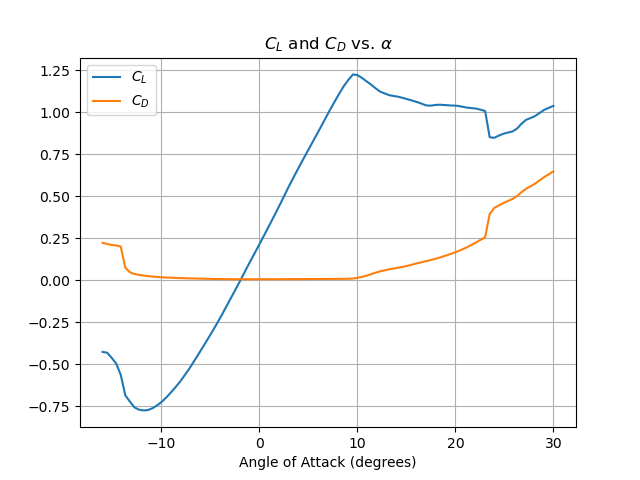
\includegraphics[width=0.6\textwidth]{Figures/CLCD_interpolation.png}
    \caption{Lift Curve and Drag}
    \label{fig:lift curve and drag}
\end{figure}

\section{Corrections}
\begin{figure}[H]
    \centering
    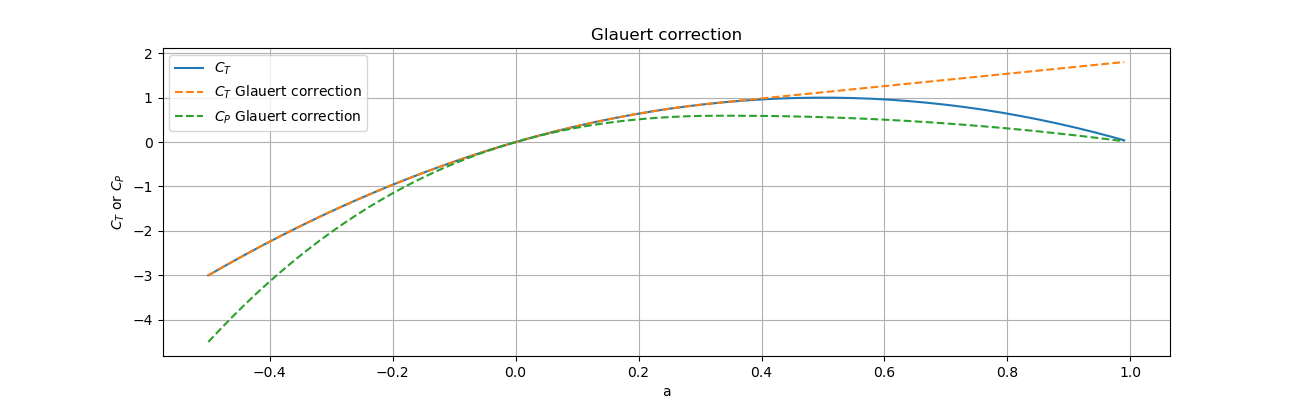
\includegraphics[width=\textwidth]{Figures/Glauert_correct.png}
    \caption{Glauert correction}
    \label{fig:glauert correction}
\end{figure}
\begin{figure}[H]
    \centering
    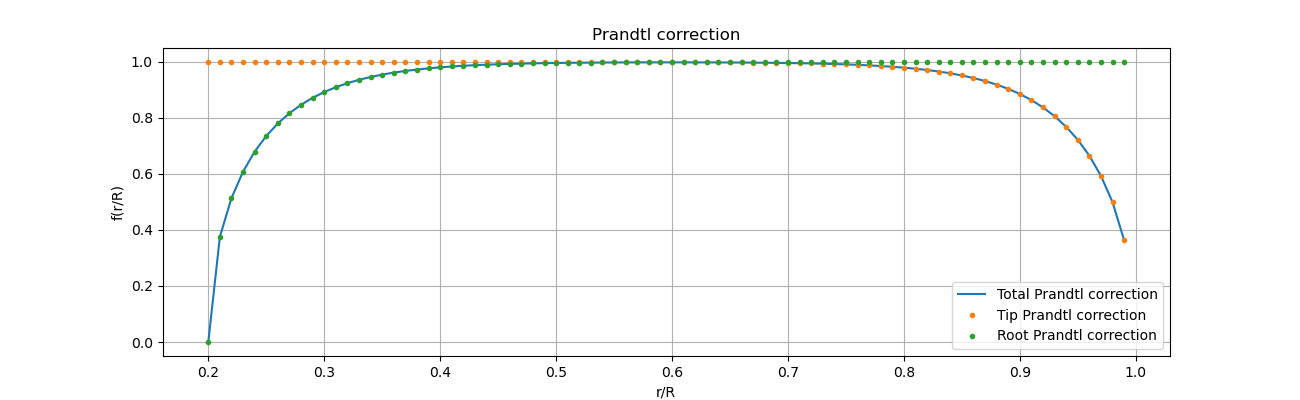
\includegraphics[width=\textwidth]{Figures/prandtl_correct.png}
    \caption{Prandtl correction}
    \label{fig:prandtl correction}
\end{figure}

\section{Angles}
\begin{figure}[H]
    \centering
    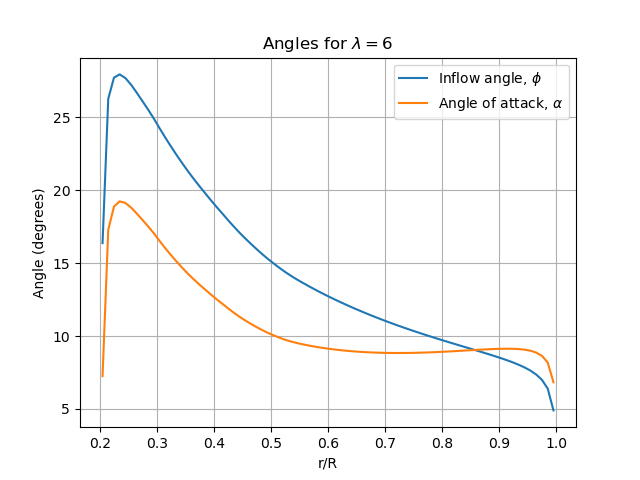
\includegraphics[width=0.6\textwidth]{Figures/alpha_phi_6.png}
    \caption{Spanwise distribution of Angle of Attack and Inflow Angle for Tip Speed Ratio of 6}
    \label{fig:spanwise distribution of angle of attack and inflow angle - lambda 6}
\end{figure}
\begin{figure}[H]
    \centering
    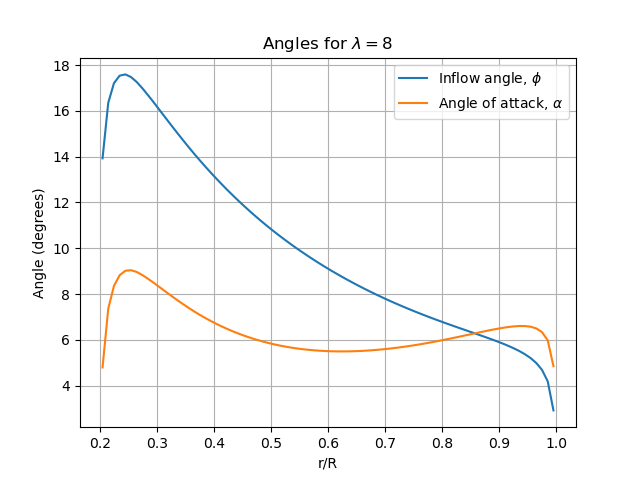
\includegraphics[width=0.6\textwidth]{Figures/alfa_phi_8.png}
    \caption{Spanwise distribution of Angle of Attack and Inflow Angle for Tip Speed Ratio of 8}
    \label{fig:spanwise distribution of angle of attack and inflow angle - lambda 8}
\end{figure}
\begin{figure}[H]
    \centering
    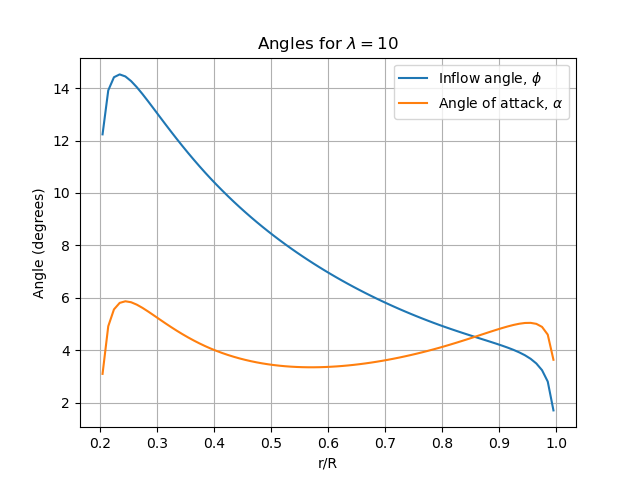
\includegraphics[width=0.6\textwidth]{Figures/alfa_phi_10.png}
    \caption{Spanwise distribution of Angle of Attack and Inflow Angle for Tip Speed Ratio of 10}
    \label{fig:spanwise distribution of angle of attack and inflow angle - lambda 10}
\end{figure}

\section{Induction factors}
\begin{figure}[H]
    \centering
    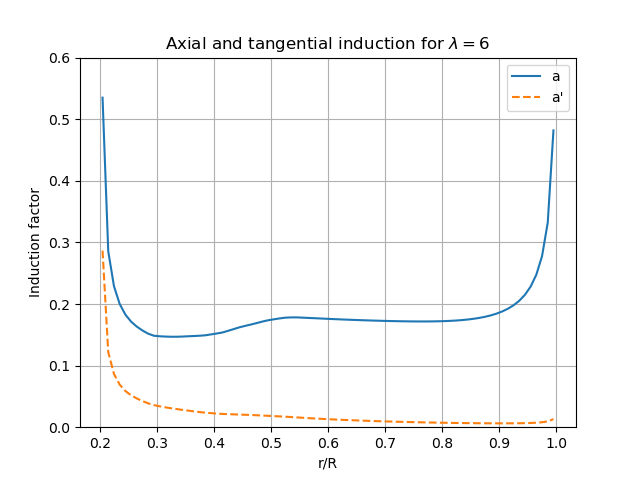
\includegraphics[width=0.6\textwidth]{Figures/a_a_prime_6.png}
    \caption{Caption}
    \label{fig:enter-label}
\end{figure}
\begin{figure}[H]
    \centering
    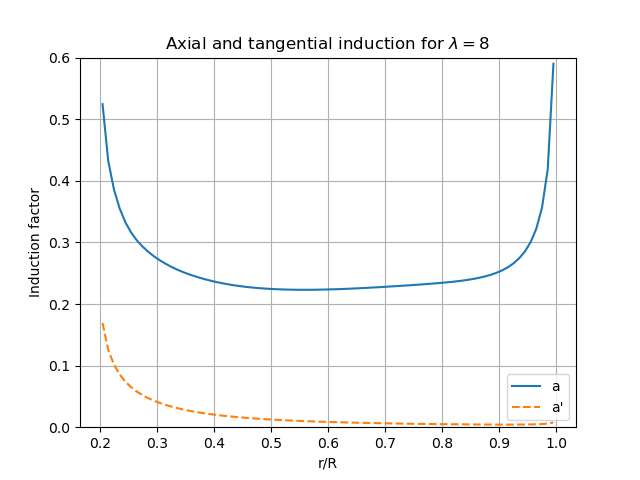
\includegraphics[width=0.6\textwidth]{Figures/a_a_p_8.png}
    \caption{Caption}
    \label{fig:enter-label}
\end{figure}
\begin{figure}[H]
    \centering
    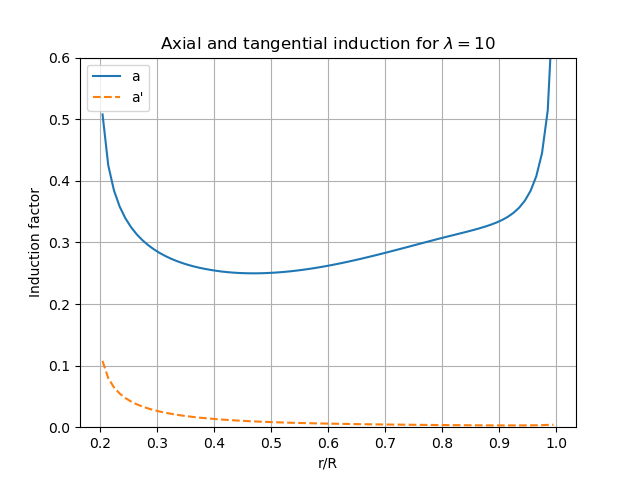
\includegraphics[width=0.6\textwidth]{Figures/a_a_p_10.png}
    \caption{Caption}
    \label{fig:enter-label}
\end{figure}


\section{Forces}
\begin{figure}[H]
    \centering
    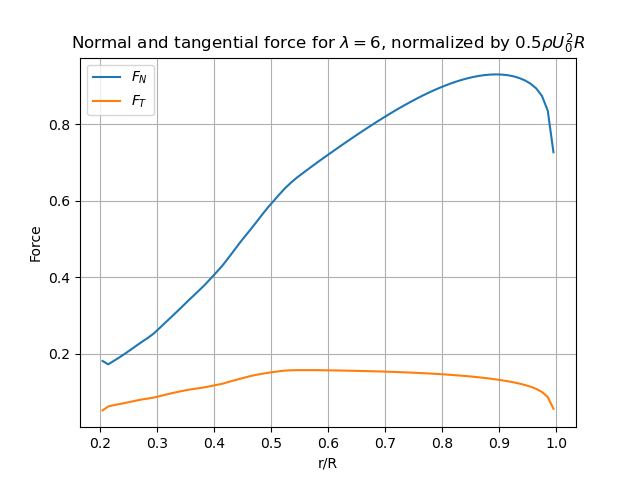
\includegraphics[width=0.6\textwidth]{Figures/F_t_F_n_6.png}
    \caption{Caption}
    \label{fig:enter-label}
\end{figure}\begin{figure}[H]
    \centering
    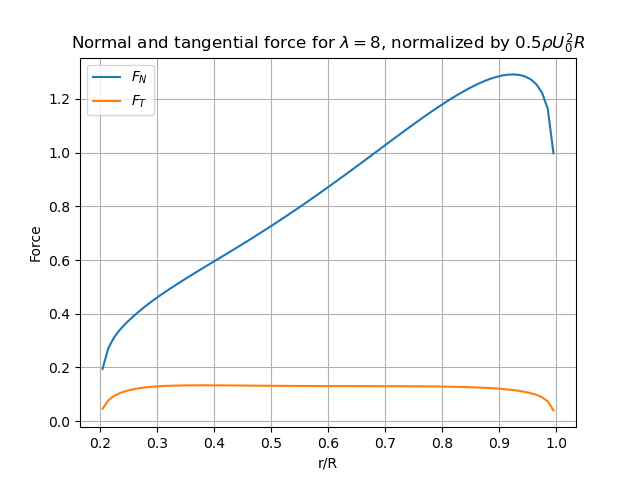
\includegraphics[width=0.6\textwidth]{Figures/Ft_Fn_8.png}
    \caption{Caption}
    \label{fig:enter-label}
\end{figure}\begin{figure}[H]
    \centering
    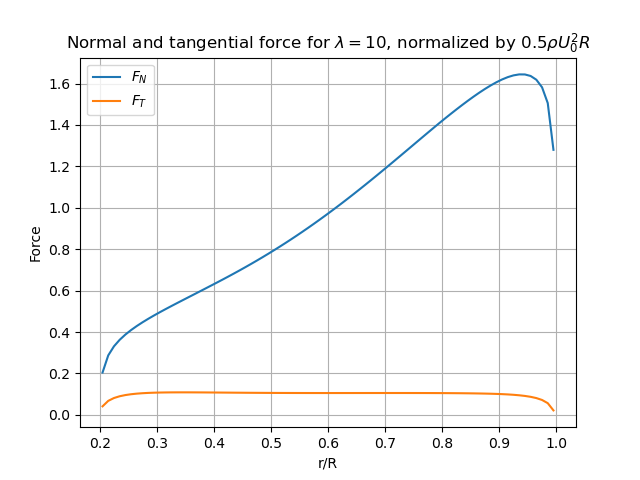
\includegraphics[width=0.6\textwidth]{Figures/Ft_Fn_10.png}
    \caption{Caption}
    \label{fig:enter-label}
\end{figure}

\section{Circulation}
\begin{figure}[H]
    \centering
    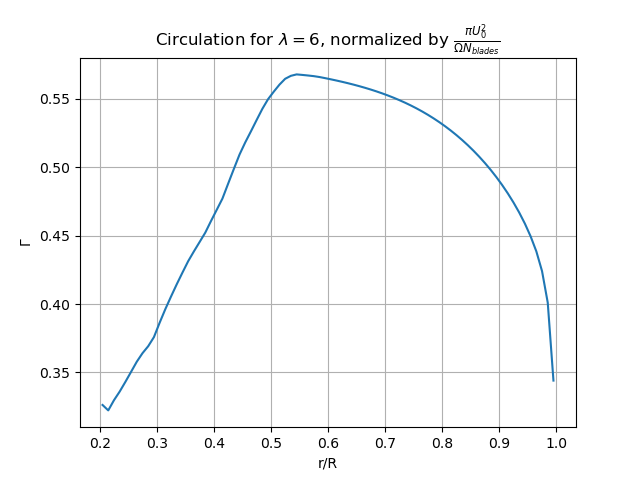
\includegraphics[width=0.6\textwidth]{Figures/Circulation_6.png}
    \caption{Caption}
    \label{fig:enter-label}
\end{figure}
\begin{figure}[H]
    \centering
    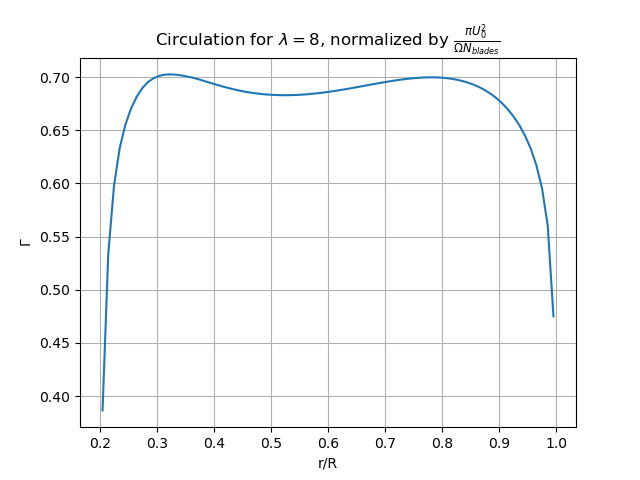
\includegraphics[width=0.6\textwidth]{Figures/Circulation_8.png}
    \caption{Caption}
    \label{fig:enter-label}
\end{figure}
\begin{figure}[H]
    \centering
    \includegraphics[width=0.6\textwidth]{Figures/Circulation_10.png}
    \caption{Caption}
    \label{fig:enter-label}
\end{figure}

\section{static pressure}
\begin{figure}[H]
    \centering
    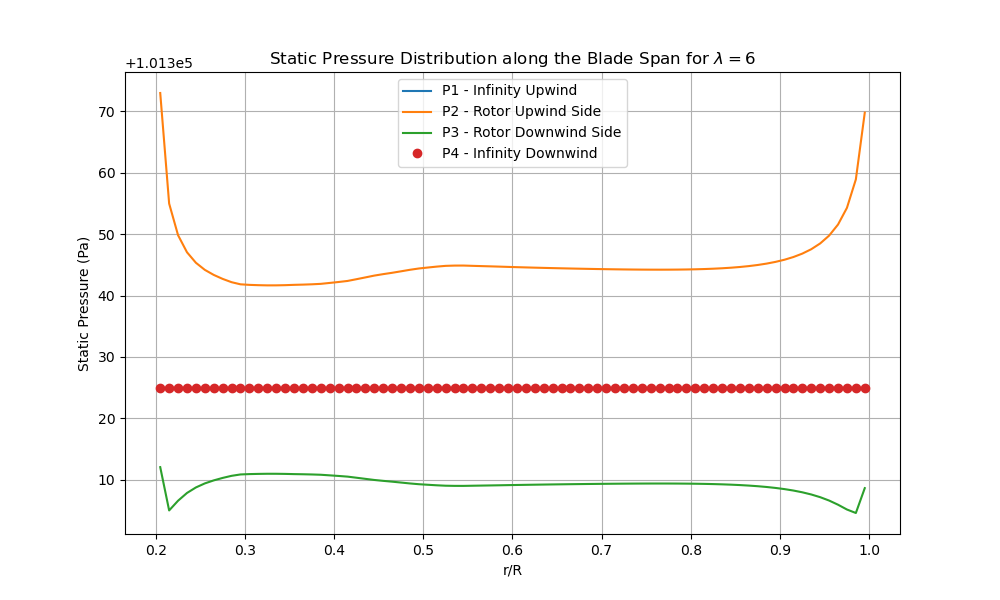
\includegraphics[width=0.6\textwidth]{Figures/pres_static_6.png}
    \caption{Caption}
    \label{fig:enter-label}
\end{figure}
\begin{figure}[H]
    \centering
    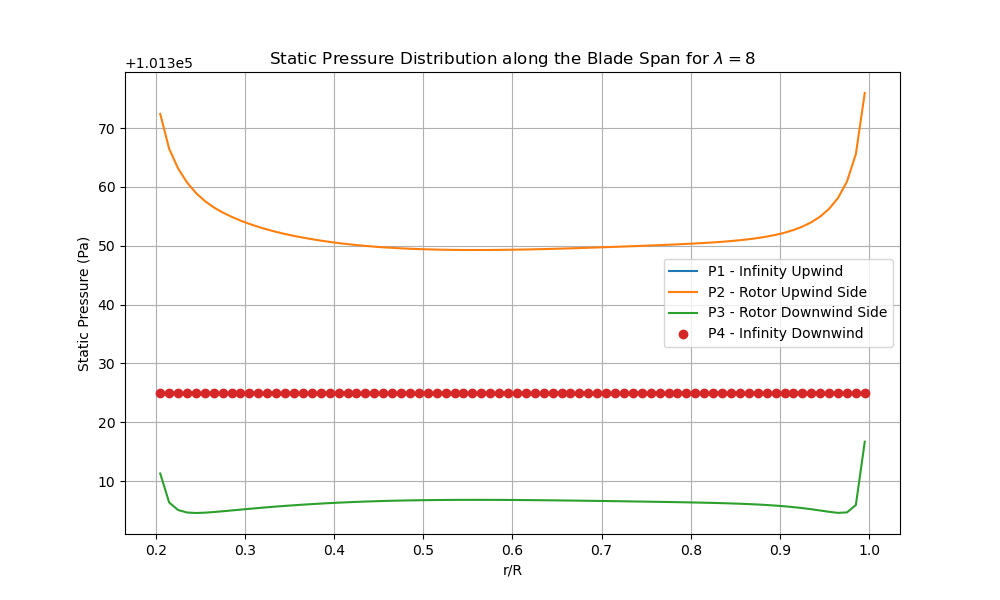
\includegraphics[width=0.6\textwidth]{Figures/pres_static_8.png}
    \caption{Caption}
    \label{fig:enter-label}
\end{figure}
\begin{figure}[H]
    \centering
    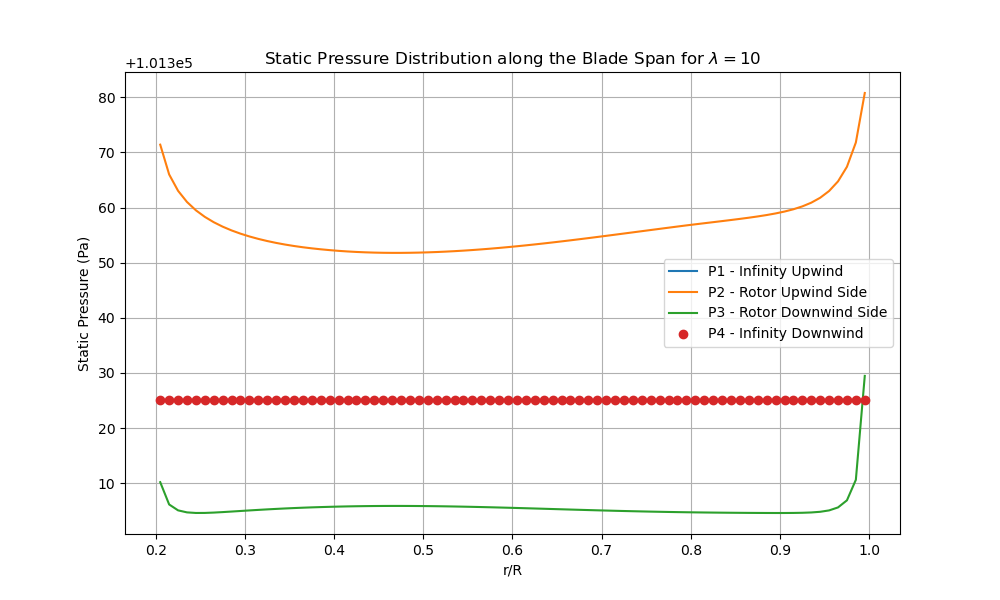
\includegraphics[width=0.6\textwidth]{Figures/pres_static_10.png}
    \caption{Caption}
    \label{fig:enter-label}
\end{figure}

\section{Total pressure}
\begin{figure}[H]
    \centering
    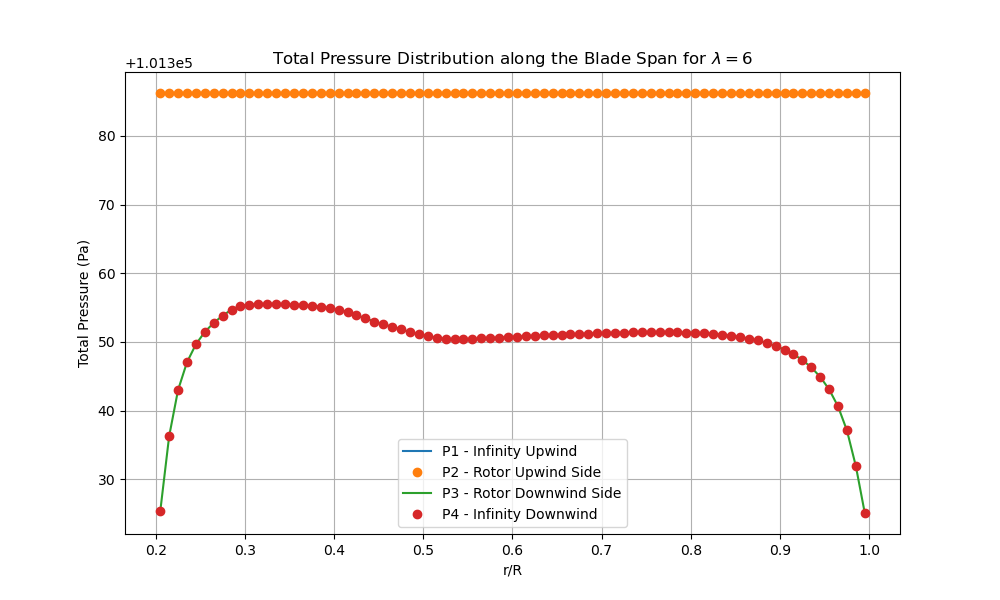
\includegraphics[width=0.6\textwidth]{Figures/pres_total_6.png}
    \caption{Caption}
    \label{fig:enter-label}
\end{figure}
\begin{figure}[H]
    \centering
    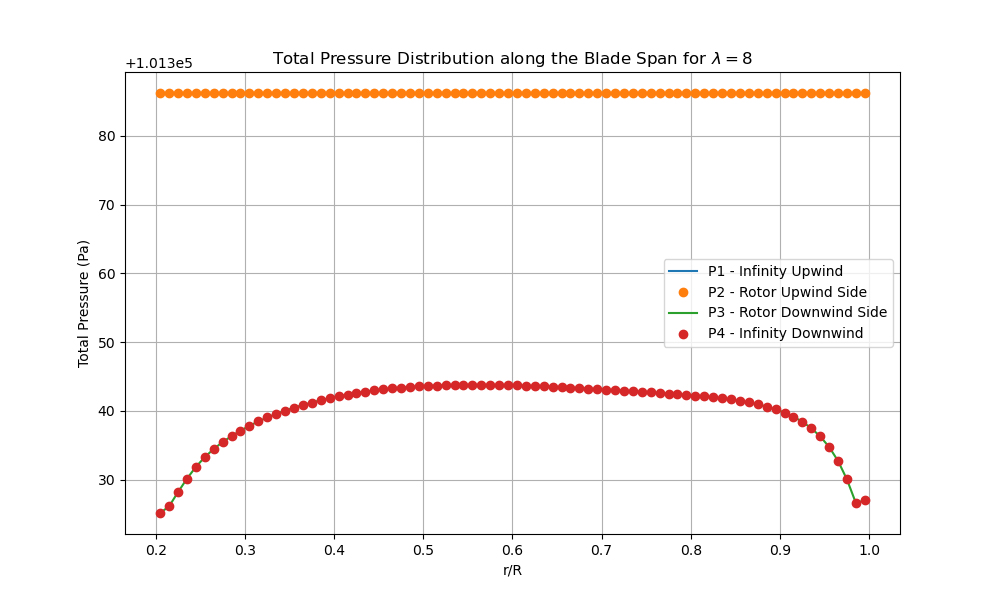
\includegraphics[width=0.6\textwidth]{Figures/pres_total_8.png}
    \caption{Caption}
    \label{fig:enter-label}
\end{figure}
\begin{figure}[H]
    \centering
    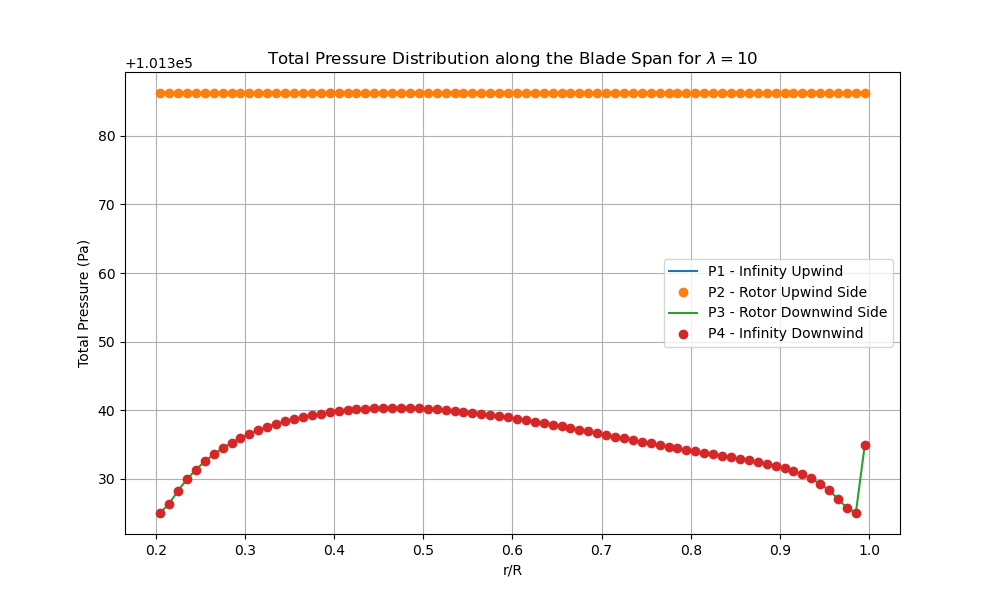
\includegraphics[width=0.6\textwidth]{Figures/pres_total_10.png}
    \caption{Caption}
    \label{fig:enter-label}
\end{figure}

\section{Thrust and torque vs TSR}
\begin{figure}[H]
    \centering
    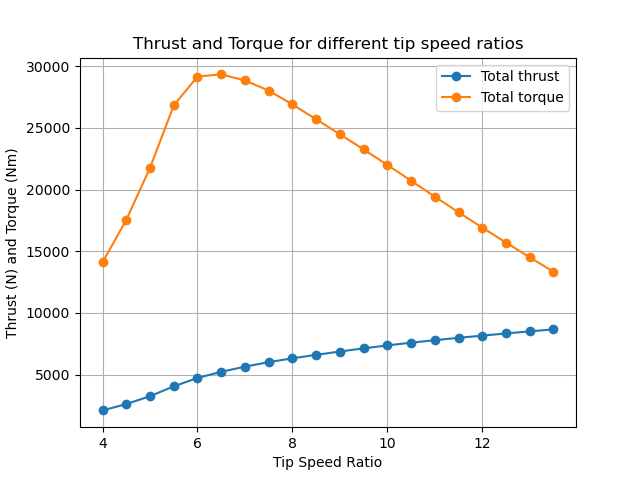
\includegraphics[width=0.8\textwidth]{Figures/Thrust_torque_TSR.png}
    \caption{Caption}
    \label{fig:enter-label}
\end{figure}

\section{Thrust vs number of annuli}
\begin{figure}[H]
    \centering
    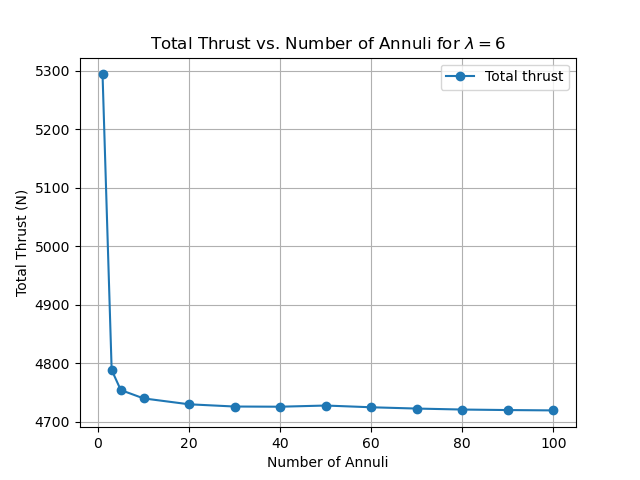
\includegraphics[width=0.6\textwidth]{Figures/annuli_6.png}
    \caption{Caption}
    \label{fig:enter-label}
\end{figure}
\begin{figure}[H]
    \centering
    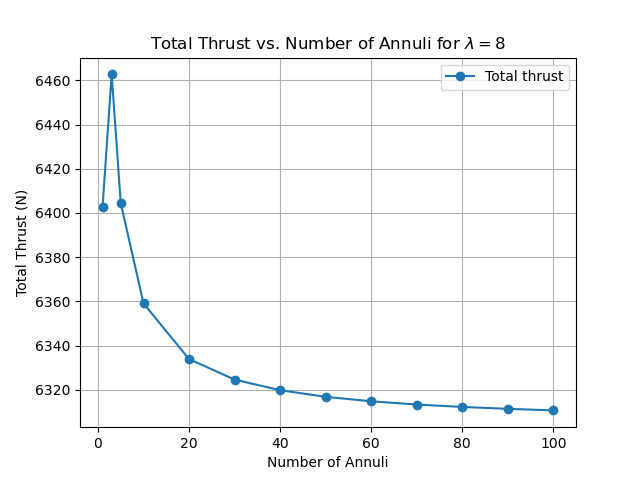
\includegraphics[width=0.6\textwidth]{Figures/annuli_8.png}
    \caption{Caption}
    \label{fig:enter-label}
\end{figure}
\begin{figure}[H]
    \centering
    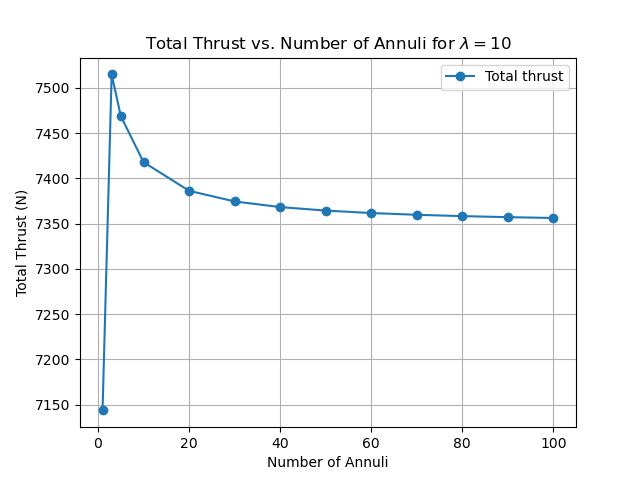
\includegraphics[width=0.6\textwidth]{Figures/annuli_10.png}
    \caption{Caption}
    \label{fig:enter-label}
\end{figure}

\section{Effect of spacing method on convergence}
\begin{figure}[H]
    \centering
    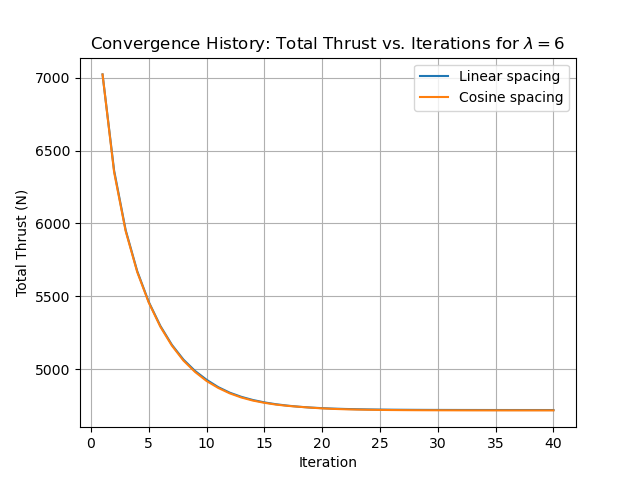
\includegraphics[width=0.6\textwidth]{Figures/Spacing_method_6.png}
    \caption{Caption}
    \label{fig:enter-label}
\end{figure}
\begin{figure}[H]
    \centering
    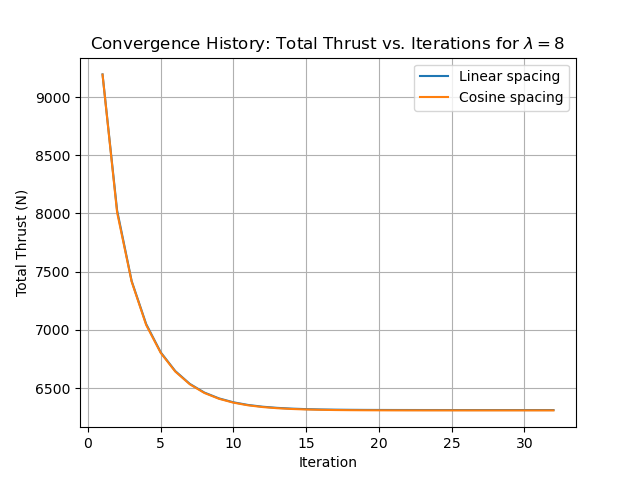
\includegraphics[width=0.6\textwidth]{Figures/spacing_method_8.png}
    \caption{Caption}
    \label{fig:enter-label}
\end{figure}
\begin{figure}[H]
    \centering
    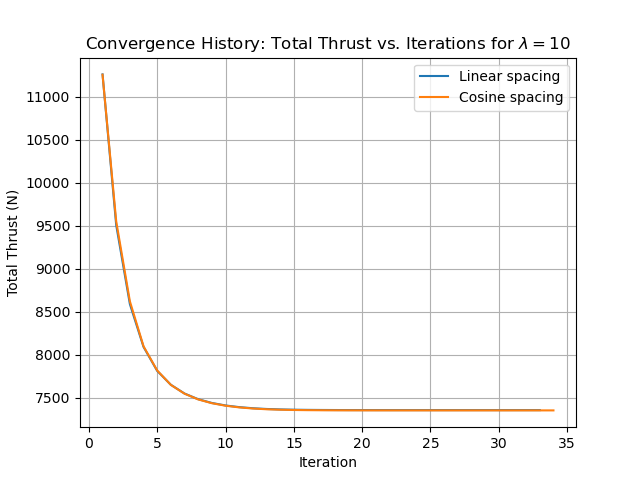
\includegraphics[width=0.6\textwidth]{Figures/spacing_method_10.png}
    \caption{Caption}
    \label{fig:enter-label}
\end{figure}